\documentclass[preprint,review,12pt]{article}			% Double line spacing
\usepackage[a4paper,margin=3cm]{geometry}
\usepackage{amsmath,amssymb,amsthm}
\usepackage{graphicx,float}
\usepackage[sort&compress,square,numbers]{natbib}			% Bibliography
\usepackage{decimal}
\usepackage{lineno}
\usepackage[labelfont=bf,width=\textwidth,nooneline,normalsize]{caption} 		

\begin{document}

%\begin{frontmatter}

\title{Can HIV epidemics among men who have sex with men be eliminated through participation to PrEP rollouts?}
 
%\author[a]{Sof\'ia Jij\'on}
%\address[a]{Sorbonne Universit\'e, INSERM, Institut Pierre Louis d'\'Epid\'emiologie et de Sant\'e Publique (IPLESP UMR-S 1136), 75012 Paris, France.}
%
%\author[b]{Jean-Michel Molina}
%\address[b]{D\'epartement de Maladies Infectieuses, APHP-H\^opital Saint Louis, UMR~941 Inserm et Sorbonne Paris Cit\'e, Paris, France.}
%%\ead{jean-michel.molina@aphp.fr}
%
%\author[a]{Dominique Costagliola}
%%\ead{dominique.costagliola@iplesp.upmc.fr}
%
%\author[a]{Virginie Supervie}
%%\ead{virginie.supervie@inserm.fr}
%
%\author[c]{Romulus Breban\corref{correspondingauthor}}
%\address[c]{Institut Pasteur, Unit\'e d'Epid\'emiologie des Maladies Emergentes, 75015 Paris, France.}
%\ead{romulus.breban@pasteur.fr}
%
%\cortext[correspondingauthor]{Corresponding author}

\maketitle 
% ABSTRACT


%\begin{abstract}

\paragraph{Objectives}
To study the conditions under which PrEP coverage can eliminate HIV among men who have sex with men (MSM) in the Paris region. 

\paragraph{Design} 
Mathematical modeling.

\paragraph{Methods}
We propose an innovative approach, combining a transmission model with a game-theoretic model, for decision-making about PrEP use. Individuals at high risk of HIV infection decide to use PrEP, depending on their perceived risk of infection and the relative cost of using PrEP versus antiretroviral treatment (ART), which includes monetary and/or non-monetary aspects, such as price and access model of PrEP, consequences of being infected and lifelong ART. 

\paragraph{Results}
If individuals perceive fairly their infection risk, and the cost of using PrEP is sufficiently low, the PrEP coverage can lead to elimination. Specifically, assuming 86\% PrEP effectiveness, as observed in two clinical trials, a minimum PrEP coverage of 55\% (95\% CI:43\%--64\%) among high-risk MSM would achieve elimination in the Paris region. A complete condom drop by PrEP users slightly increases the minimum PrEP coverage by $\sim$1\%, while underestimation of their own HIV infection risk would demand PrEP programs to reduce the cost of using PrEP by a factor $\sim$2 to achieve elimination. 
 
\paragraph{Conclusions}
Elimination conditions are not yet met in the Paris region, where at most 47\% of high-risk MSM were using PrEP as of mid-2019. Further lowering the cost of PrEP and promoting a fair perception of HIV risk are required and should be maintained in the long run, to maintain elimination status.

%\end{abstract}
%
%\begin{keyword}
%Pre-exposure prophylaxis; HIV; men who have sex with men; behavioral epidemiology; game theory.\end{keyword}

Word count:
Abstract: 247/250
Main text: 3498/3500
 

%\end{frontmatter}

\linenumbers
\modulolinenumbers[5]



\section{Introduction} \label{sec:Intro}

In many settings, men who have sex with men (MSM) are the most affected by HIV.\cite{Beyrer2016} Pre-exposure prophylaxis (PrEP) is a highly effective prevention method recommended by the WHO for individuals at high risk of infection with HIV [2]. Both IPERGAY and PROUD clinical trials showed that PrEP can reduce HIV incidence among MSM by $86\%$.\cite{Molina2015,McCormack2016} Modeling studies elaborating on these results suggested that PrEP has the potential to curtail, and even eliminate, HIV epidemics, notably among MSM.\cite{Jenness2016,Rozhnova2018,Hansson2020,Scott2018} For instance, it was found that, in the United States (US), a $40\%$ PrEP coverage, among high-risk MSM, would lead to a $33\%$ decrease in the number of new HIV infections, ten years after PrEP initiation.\cite{Jenness2016} In the Netherlands, HIV elimination would require $82\%$ PrEP coverage in the highest-risk group.\cite{Rozhnova2018} Furthermore, in Sweden, a PrEP coverage of at least $10\%$ for the sexually high active MSM could reduce HIV prevalence to nearly $0\%$ in the long term.\cite{Hansson2020}

PrEP represents a promising prevention option, bringing new hope to end HIV epidemics. Yet, the question of how to achieve a certain PrEP coverage in a population has never been addressed; the coverage is only assumed to reach certain values, which may not be granted in practice. It is therefore unclear whether and how target PrEP coverage levels, required to substantially impact or eliminate HIV epidemics, can be reached and maintained in the long term. As of October 2019, PrEP was approved by regulatory agencies in more than 40 countries,\cite{PrEPwatch_2019} but only a few settings strongly promoted it.\cite{Cohen2018} In the US, $130\,000$--$135\,000$ individuals were on PrEP as of October 2019.\cite{PrEPwatch_2019} This represents $\sim34\%$ of the worldwide PrEP users,\cite{PrEPwatch_2019} still falling short of the CDC estimate that $1.2$ million persons in the US have indications to consider PrEP use.\cite{Laufer2015} Furthermore, a recent US study shows that only two in five individuals keep using PrEP for more than two years.\cite{Coy2019} Hence, PrEP remains underutilized in many settings.

Mathematical tools for qualitative and quantitative analyses of individual-level decision-making are offered by game theory.\cite{Verelst2016,Manfredi2017} We propose an innovative approach, combining a compartmental model of HIV transmission at the population level, and a game-theoretic model for decision-making about PrEP at the individual level. We model PrEP adoption in a population at high risk of HIV infection to determine whether and how certain PrEP coverage levels can be reached. Particularly, we study the potential impact of PrEP among MSM in the Paris region of France, where universal antiretroviral treatment (ART) is in place, and PrEP is available for individuals meeting eligibility criteria. The HIV epidemiology among MSM in the Paris region is similar to those of other urban settings in high-income countries.\cite{Marty2019}


\section{Methods} \label{sec:Methods}

\subsection{The mathematical model} \label{subsec:MathModel}

We built an HIV transmission model to describe the epidemiological context where individuals meeting eligibility criteria make their decision on PrEP adoption. We assumed that individuals have a certain perception of the risk of infection and make their decisions by judging pros and cons of PrEP and ART. According to game theory, such a process can be modeled as a non-cooperative game, where individuals act in their own interest to maximize the utility of adopting PrEP, or, in other words, minimize the cost of using PrEP to later avoid using ART. However, an individual's decision is indirectly influenced by those of others. The sum of all individuals' decisions determines the proportion of the population that uses PrEP, which, in turn, affects the epidemic progression and the probability of acquiring infection. The game model is thus intertwined with the epidemic model. Below, we describe the main features and assumptions of our two-component model; see appendix section~1 for details. 

\subsubsection{Modeling HIV transmission in an MSM population} \label{subsec:TransmissionModel}

The transmission model is compartmental, using ordinary differential equations. The MSM population is stratified into two risk groups (low and high) to account for heterogeneity in risk of HIV infection;\cite{Jacquez1989} high-risk individuals have a higher number of sexual partners and a higher risk of acquiring HIV than low-risk individuals. The majority of partnerships occur within the same risk group (i.e., non-random mixing)\cite{Jacquez1988} and individuals at high risk of infection drive the epidemic.\cite{Lions2019} The model compartments represent susceptible individuals who are on or off PrEP, HIV-infected individuals who are unaware of their HIV status, and those diagnosed and undergoing ART. Once diagnosed, individuals immediately begin ART, no longer transmitting HIV; that is, only infected individuals unaware of their status transmit HIV. Only susceptible individuals at high risk of infection are eligible for PrEP and, once on PrEP, they use condoms less frequently.\cite{Molina2018} We varied the PrEP effectiveness, denoted $\varepsilon$, from $0$ to $100\%$ to account for sub-optimal PrEP adherence. The PrEP coverage, denoted $p$, was not fixed; rather, it was obtained by solving the decision-making model; see next section.

We computed the effective reproduction number, $R$, defined as the expected number of secondary HIV infections caused by a single infected individual, during his entire infectious period, in an uninfected population subject to control interventions (e.g., condom use before the introduction of PrEP).\cite{Jacquez1988,VandenDriessche2002} The introduction of PrEP may change individual's preference for condom use, and adds PrEP parameters to the HIV prevention profile. Hence, $R$ becomes a function of PrEP coverage and effectiveness, denoted $R(p,\varepsilon)$. The effective reproduction number measures how close the epidemic is to elimination. $R(p,\varepsilon)>1$ indicates self-sustained transmission and persistence of the epidemic, meaning that an endemic state will be reached. Epidemic elimination requires $R(p,\varepsilon)<1$, such that the disease-free state is reached. Thus, HIV incidence is reduced to zero in some communities, but HIV can re-emerge in absence of control interventions. We say that the epidemic is controlled through the use of PrEP if $R(p,\varepsilon)$ decreases due to the introduction of PrEP, although the decrease is not below 1.

Our transmission model shows that HIV elimination is possible, provided that prevention parameters exceed certain values. We identified two thresholds for PrEP effectiveness: $\varepsilon \geq \varepsilon_{\rm C}$ is required for PrEP to contribute to epidemic control and $\varepsilon \geq \varepsilon_{\rm E}$ is required for PrEP to eliminate the epidemic. We call these thresholds in $\varepsilon$ the epidemic control threshold and the epidemic elimination threshold, respectively; see appendix section~1.2.3 for details. It is important to note that reaching these thresholds is necessary, but not sufficient, to achieve epidemic control and elimination, respectively. 


\subsubsection{The individual-level decision-making on PrEP adoption} \label{subsec:DecisionModel}

During an epidemic, individuals may adopt PrEP according to how they perceive the risk of infection,\cite{Bull2018} the consequences of being infected, the price and access model of PrEP,\cite{Gilson2018} undesired secondary effects,\cite{Thomann2017} social stigma,\cite{Brooks2019} and other pros and cons. These factors, summarizing monetary and/or non-monetary aspects, are expressed in the decision-making model as costs perceived by the individual. 

We assume that each individual makes his decision at the beginning of his sexual mixing period, opting for one of two independent strategies. If an individual decides not to use PrEP, he will start treatment upon positive HIV diagnosis, and pay the cost of ART for the rest of his life; we use the notation $C_{\text{\tiny No-PrEP}}$ for the lifetime cost of this strategy. Otherwise, the individual decides to adopt PrEP prevention, he takes and pays the cost of PrEP and, in the case of acquiring HIV despite PrEP uptake, being diagnosed and starting ART, he pays the cost of treatment for the rest of his life; we use the notation $C_{\text{\tiny PrEP}}$ for the lifetime cost of the second strategy. Hence, the total cost depends explicitly on the yearly cost of treatment and cost of PrEP, the PrEP parameters, and, implicitly, the yearly risk of acquiring HIV; see appendix section~1.3.2 for details. Introducing $r$, the relative cost of PrEP versus ART, the balance of cost, when the probability to adopt PrEP is $p$, is given by 
\begin{equation} \label{eq:C}
	C(p,\varepsilon, r) = p \, C_{\text{\tiny PrEP}}(p,\varepsilon, r) + (1- p) \, C_{\text{\tiny No-PrEP}}(p,\varepsilon).
\end{equation}
The particular value of $p$ that minimizes the total expected cost $C(p,\varepsilon, r)$, denoted $\hat{p}(\varepsilon, r)$, provides an estimate of the probability that a typical high-risk individual decides to use PrEP, and also represents the voluntary PrEP coverage among high-risk MSM. The solution of the game represents a long-term equilibrium where individuals make decisions to adopt PrEP in stationary epidemiological context. Hence, we assume that individuals maintain their decisions about adopting PrEP.


\subsubsection{Application to the HIV epidemic among MSM in the Paris region} \label{subsec:Paris}

We applied our model to the population the most at risk of HIV infection in mainland France: MSM in the Paris region, \^Ile-de-France. Surveillance data collected before 2016, when PrEP was introduced, suggested that the HIV epidemic was close to an endemic state, where epidemiological indicators remain nearly constant.\cite{Marty2019,RapportSPF2019} We used latin hypercube sampling and bootstrap techniques to generate parameter sets and selected those which calibrated the HIV transmission model to the endemic state in 2016;\cite{Marty2019} see appendix section~2. In turn, these parameter sets revealed uncertainties in the model outputs and allowed estimation of confidence intervals.

In our baseline scenario, we assumed that MSM on PrEP get tested for HIV infection every three months, according to the recommendation in France,\cite{CNSANRS2018} and most countries where PrEP is available. It is important to note that this testing frequency on PrEP is much higher than the testing frequency among MSM before the introduction of PrEP, when the median time from HIV infection to diagnosis for MSM was $3.1$ years~\cite{Marty2019}. Therefore, the introduction of PrEP has a dual effect on the HIV epidemiology: first, it offers the prevention benefits of the regimen, and, second, it acts as a test-and-treat strategy\cite{Kretzschmar2013,WHO2016} due to the dramatic change in HIV testing practice. 

We further assumed that individuals have a fair sense of their risk of infection when making decisions about PrEP use. The risk of infection corresponds to the force of HIV infection and was computed using the transmission model. MSM dropped condom use from $30\%$ to $20\%$ when adopting PrEP,\cite{Molina2015} and condom effectiveness was set at $58\%$--$80\%$.\cite{Smith2015} We performed sensitivity analyses, assuming that i) MSM misperceive their risk of HIV infection, ii) MSM adopting PrEP completely drop condom use, or iii) MSM do not change their HIV testing behavior when adopting PrEP; see appendix section~3. 

\section{Results} \label{sec:Results}

About $500$ parameter sets passed the calibration filter constructed to reflect the HIV epidemiology among MSM, in the Paris region, before the introduction of PrEP: overall yearly mean incidence was $1.3\%$, mean prevalence was $17\%$, and $17\%$ of MSM living with HIV were unaware of their infection; see appendix section~2 and table~S1. The mean number of MSM was $\sim 111\,000$, of which 13\% (i.e., $\sim 14\,200$) were at high risk of HIV infection and eligible for PrEP. Yearly mean HIV incidence for high-risk MSM was $7\%$. 


\subsection{The voluntary PrEP coverage if individuals perceived correctly HIV risk} \label{subsec:VoluntaryPrEP} 
 
We first did computations for a typical parameter set calibrating our model. The PrEP coverage starts at zero, before introducing PrEP, and then reaches an optimal value where the expected cost of adopting PrEP is minimum. The final value reached depends on HIV parameters of the epidemic before the introduction of PrEP, the PrEP effectiveness, $\varepsilon$, and the perceived relative cost of PrEP versus ART, $r$. The color map in figure~\ref{fig:1}A shows the voluntary PrEP coverage reached among high-risk MSM, $\hat{p}(\varepsilon,r)$, as function of $\varepsilon$ and $r$. Figure~\ref{fig:1}B shows the corresponding relative reduction in the overall HIV incidence in the MSM community. We identified three regions on each color map:

\begin{itemize}
\item Region~III, where no high-risk MSM adopts PrEP for HIV prevention (i.e., $\hat{p}=0\%$), because 
the relative cost of PrEP versus ART, perceived by the individuals, is too high. Therefore, HIV remains endemic, unaffected by the introduction of PrEP (i.e., no reduction in incidence).

\item Region~II, where some, but not enough, high-risk MSM adopt PrEP since the relative cost remains high. The epidemic is controlled and incidence decreases, but not enough for HIV elimination (i.e., $R(\hat{p},\varepsilon)>1$).

\item Region~I, where PrEP is offered at low relative cost. This allows reaching high levels of PrEP coverage ($\sim 54$--$75\%$) and the epidemic can be eliminated; in region~I, $R(\hat{p},\varepsilon)<1$. It is important to note that HIV elimination for low PrEP effectiveness (bottom part of figure~\ref{fig:1}A) occurs as a consequence of the test-and-treat effect of the PrEP rollout; consequently, the thresholds in PrEP effectiveness, to achieve epidemic control and elimination, are zero ($\varepsilon_{\rm C}= \varepsilon_{\rm E}= 0\%$). In this case, most MSM taking PrEP acquire HIV despite PrEP uptake. However, they are diagnosed and treated very early in the course of infection, because on-PrEP MSM get tested for HIV every three months. Early diagnosis and treatment prevent further HIV transmission. In contrast, when PrEP effectiveness is high (top part of figure~\ref{fig:1}A), most on-PrEP MSM do not acquire HIV, and thus do not transmit HIV, so the test-and-treat effect of the PrEP rollout is only marginal. It is PrEP, particularly its high effectiveness, that contributes decisively to epidemic elimination. 
\end{itemize}
 
It is thus possible to reach the PrEP coverage levels required to eliminate HIV, provided that the perceived relative cost of PrEP versus treatment is low. In particular, for a PrEP effectiveness of $86\%$, as observed in the IPERGAY and PROUD clinical trials, a minimum PrEP coverage of $56\%$ among the high-risk MSM is required to achieve epidemic elimination in the Paris region. However, it is important to note that elimination is temporary, as the disease-free state is unstable. Indeed, once the epidemic is eliminated, individuals' perception of HIV risk changes. The effectiveness of PrEP remains high, but the risk of HIV infection is perceived as being low. Individuals could then perceive less PrEP-induced advantages and more PrEP-induced disadvantages, that may severely increase the relative cost of PrEP versus ART. As fewer individuals will pay the cost of PrEP, the coverage decreases. Hence the epidemic dynamics in region~I (i.e., the elimination region) can enter region~II (i.e., the control region), where an endemic state can be reached, again.

\begin{figure}[H] 
	\centering	
	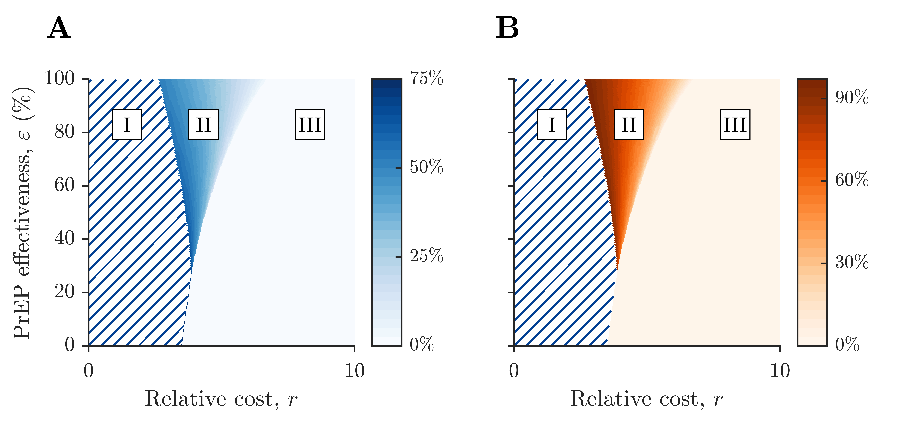
\includegraphics{Figures/Fig_1}
	\caption{{\bf The voluntary PrEP coverage and its impact on HIV incidence, assuming fair risk perception} \\
	Color maps of (A) the voluntary PrEP coverage among high-risk MSM, $\hat{p}$, and (B) the corresponding reduction in the overall endemic HIV incidence rate, as functions of $\varepsilon$ and $r$, assuming that individuals have a fair sense of HIV risk. The model outputs were obtained for one typical parameter set calibrating our model. Three regions were identified, depending on $\hat{p}$: region~III, where $r$ is high and no MSM uses PrEP ($\hat{p}=0\%$), so HIV incidence is not reduced; region~II, where some, but not enough MSM use PrEP, since $r$ remains high, and thus the epidemic is controlled; and region~I (marked by blue stripes), where epidemic elimination is possible.}
	\label{fig:1}
\end{figure}

We generated the outputs illustrated in figure~\ref{fig:1} for each of the $\sim500$ calibrated parameter sets to reveal the role of parameter uncertainties and obtain uncertainty intervals for our results. Figure~\ref{fig:2}A shows the probability that HIV is eliminated, as a function of PrEP effectiveness and perceived relative cost of PrEP versus ART. The probability takes high values on the left, where region~I is found, and declines severely toward region~II. In figure~\ref{fig:2}B, we illustrate the boundaries between regions~I and II (continuous line), and between regions~II and~III (dashed line). The three-region structure in figure~\ref{fig:1} is thus robust to parameter uncertainties. In addition, we found that for $86\%$ PrEP effectiveness, a minimum PrEP coverage of $55\%$ (95\%~CI: $43\%$--$64\%$) is required among high-risk MSM, for the HIV epidemic dynamics to reach region~I.

\begin{figure}[H]
	\centering
	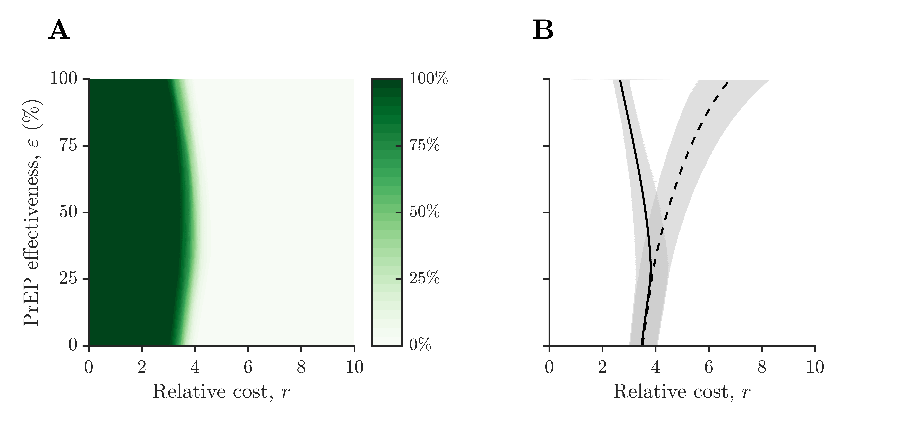
\includegraphics{Figures/Fig_2}
	\caption{{\bf The probability of HIV elimination and boundary uncertainty for the three-regions structure}\\
	(A) The probability of HIV epidemic elimination due to voluntary PrEP coverage, obtained from the $\sim500$ calibrated parameter sets. (B) The boundaries (the mean is represented as a line and the 95\%~confidence interval as grey area) between regions~I and~II (continuous line), and between regions~II and~III (dashed line).}
	\label{fig:2}
\end{figure}


\subsection{Sensitivity analyses} 
\label{subsec:SensitivityAnalyses}

We assumed that individuals could misperceive their risk of infection and, particularly, underestimate this risk when deciding to adopt PrEP, and repeated our analyses. Specifically, we assumed that, rather than having a fair sense of the risk, based on the force of infection, high-risk MSM get a sense of HIV risk from, for instance, the proportion of their high-risk MSM peers being diagnosed with HIV each year; see appendix section~3.2.1 for further details. The voluntary PrEP coverage that can be achieved under this alternative scenario is shown in figure~\ref{fig:3}A. We obtained qualitatively similar results to those in figure~\ref{fig:1}; i.e., the three-regions structure. However, when high-risk MSM misinterpret and underestimate their HIV risk, the region of the parameter space corresponding to epidemic elimination (i.e., region~I, blue stripes) is smaller, meaning that the relative cost of PrEP versus ART has to be significantly lower to reach epidemic elimination. In principle, individuals who underestimate HIV risk require a lower relative cost to adopt PrEP, than individuals who have a fair perception of risk. In particular, assuming $86\%$ PrEP effectiveness, the relative cost needed to voluntarily reach the minimum PrEP coverage required to eliminate HIV (i.e., 56\%) decreases by a factor of $\sim2$. In turn, this can place significant constraints on the cost of PrEP, making region~I harder to reach in practice. 

We performed two other sensitivity analyses. First, we analyzed PrEP-driven risk compensation and condom drop. In the baseline scenario, we considered a drop from $30\%$ to $20\%$ in the probability of using condoms for PrEP users. Qualitatively similar results were obtained assuming that PrEP users stopped using condoms completely;\cite{Holt2018} see figure S7 and appendix section~3.2.2. In this case, epidemic elimination assuming PrEP effectiveness at $86\%$ would require a coverage of at least $57\%$, rather than $56\%$ in the baseline scenario. Hence, we found that condom drop does not play an important role against HIV elimination when PrEP effectiveness is high.

Second, we analyzed a scenario where PrEP uptake does not require higher rates of HIV testing and MSM do not change their HIV testing behavior when adopting PrEP; see figure~\ref{fig:3}B and appendix section~3.2.3. In this case, we found that HIV elimination is entirely due to PrEP and can only be reached if PrEP effectiveness is above the epidemic elimination threshold $\varepsilon_{\rm E} = 58\%$. For high PrEP effectiveness, the results are very close to those of the baseline scenario, as very few individuals fail PrEP, and thus the testing frequency on PrEP does not affect the impact of the PrEP rollout. For instance, for $86\%$ PrEP effectiveness, a $58\%$ PrEP coverage, rather than $56\%$ in the baseline scenario, would be sufficient to achieve HIV elimination. For low PrEP effectiveness, the color map of the voluntary PrEP coverage versus $\varepsilon$ and $r$ figure~\ref{fig:3}B shows a fourth region, where low relative cost encourages all high-risk MSM to adopt PrEP ($\hat{p}=100\%$) and PrEP effectiveness is above the epidemic control threshold ($\varepsilon_{\rm C}= 8\%$), but below the epidemic elimination threshold ($\varepsilon_{\rm E}= 58\%$). Therefore, the epidemic is controlled, but not eliminated (i.e., $R(p,\varepsilon)>1$), and a new endemic state is reached.

\begin{figure}[H]
	\centering	
	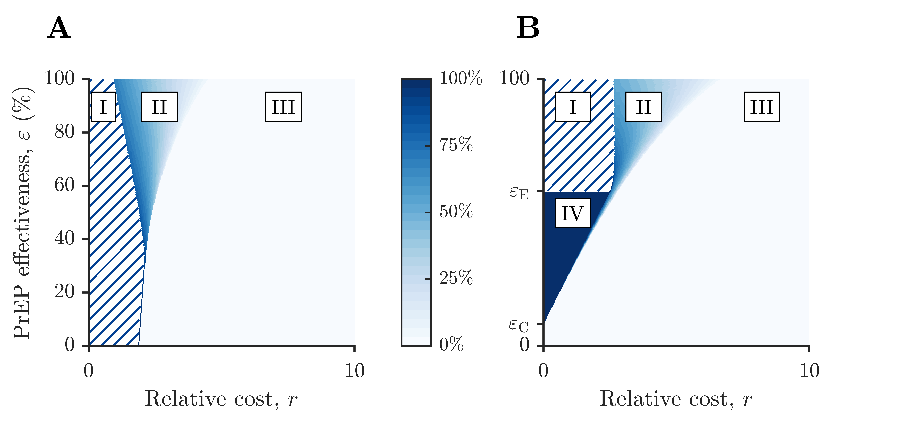
\includegraphics{Figures/Fig_3}
	\caption{{\bf Sensitivity analyses for the baseline scenario}\\
	Sensitivity analyses for the baseline scenario
(A) Decision-making based on misperceived risk of acquiring HIV can significantly reduce the size of region~I, where epidemic elimination is possible (blue stripes), despite high levels of PrEP effectiveness. (B) By assuming fair perception of HIV risk but no change in HIV testing behavior among PrEP users (i.e., the time to diagnosis remains at $3.1$ years), the PrEP effectiveness thresholds required to reach epidemic control and epidemic elimination become $\varepsilon_{\rm C} = 8\%$ and $\varepsilon_{\rm E} = 58\%$, respectively. In turn, this yields a fourth region, denoted region~IV, where all individuals adopt PrEP but $\varepsilon_{\rm C} \leq \varepsilon<\varepsilon_{\rm E}$, so the epidemic is controlled but not eliminated. Regions~II and~III in both panels depict some and no PrEP adoption, respectively, similarly to figure~\ref{fig:1}A.
	}
	\label{fig:3}
\end{figure}

\subsection{Perspectives on the PrEP rollout in the Paris region} \label{subsec:ParisPerspectives}

In 2016, a PrEP rollout started in the Paris region, offering fully subsidized PrEP to qualifying individuals through specialized HIV centers. As aforementioned, for $86\%$ PrEP effectiveness, we found that at least 55\% (95\%~CI: $43\%$--$64\%$) of the high-risk MSM would need to be on PrEP for the HIV epidemic be eliminated. Since, according to our calibration, the estimated number of PrEP eligible MSM in the Paris region is $14\,200$ (95\%~CI: $9\,200$--$23\,000$), this implies that $7\,700$ (95\%~CI: $5\,800$--$10\,100$) high-risk MSM should be on PrEP. This is a goal yet to be reached. As of June 2019, $\sim 6\,700$ men were enrolled in the PrEP program of the Paris region,\cite{ANSM2019} with a marked growing trend; the 30-month drop out rate was $\sim 32\%$. \cite{Costagliola2019} Therefore, the PrEP coverage among high-risk MSM was at most $47\%$ (95\%~CI: $30\%$--$73\%$), assuming that all men on PrEP were indeed MSM at high-risk of HIV infection. If all these MSM maintain their HIV prevention practices and the PrEP coverage remains stable in the long term, our model predicts epidemic control (i.e., region~II), with a reduction of $90\%$ (95\%~CI: $81\%$--$100\%$) in HIV incidence at the new endemic state.

\section{Discussion} \label{sec:Discussion}

We addressed, for the first time, the role of individual-level decision-making to evaluate the impact of PrEP on the HIV epidemic, and determined how a certain PrEP coverage level can be reached voluntarily. We modeled the voluntary PrEP coverage among MSM at high-risk of HIV infection, as a function of PrEP effectiveness, and the relative cost of PrEP versus ART, identifying the conditions for which epidemic control or elimination are possible. We obtained four major findings for PrEP rollouts. First, HIV epidemics can be eliminated provided that the relative cost of using PrEP versus ART is sufficiently low. Second, frequent HIV testing while taking PrEP can compensate the lack of PrEP effectiveness, and act as a test-and-treat intervention. Third, HIV risk perception may play a major role for elimination, while drop in condom use among PrEP users may not. Fourth, epidemic elimination may be only temporary.

We applied our model to a typical urban area of a high-income country, the Paris region of France. Assuming a PrEP effectiveness of $86\%$, as reported by two major clinical trials, we found that at least $55\%$ (95\%~CI: $43\%$--$64\%$) of the high-risk MSM in the Paris region would need to be on PrEP to achieve HIV elimination. As of June 2019, at most $47\%$ high-risk MSM were on PrEP in the Paris region, meaning that the current protocol of the PrEP rollout did not reduce enough the cost of PrEP for epidemic elimination, so far. Still, a recent update on new HIV diagnoses in the Paris region \cite{SPF2019} by Sant\'e publique France shows that the numbers among French-born MSM decreased by 28\%, between 2015 and 2018, with no significant decrease for the other MSM. This decrease could be partly due to the PrEP rollout, which started in 2016, and, according to our modeling, should continue in the near future. In two other settings, a moderate-high PrEP coverage has been quickly reached. The region of New South Wales witnessed a rapid PrEP rollout ($\sim 9\,000$ MSM on PrEP within 2 years) during an implementation study providing PrEP for free at several sites, including public HIV and sexual health services, and private general practices with expertise in ART prescription.\cite{Grulich2018} About $41\%$ of high-risk MSM were on PrEP in Australia in 2017.\cite{Kirby2020} Since April 2018, PrEP is subsidized by the Australian government and can be prescribed by any practitioner.\cite{ASHM2018} In San Francisco, a citywide coordinated PrEP rollout, within the Getting to Zero program, strongly promoted PrEP use and allowed many people to access PrEP for free or at low monetary cost, by using their insurance benefits or patient assistance programs. Close to $50\%$ of the eligible MSM were estimated to be on PrEP in 2017, in San Francisco.\cite{SFO_2017} Although these levels of PrEP coverage contributed to decreasing HIV transmission,\cite{Grulich2018,SFO_2017,Smith2020} HIV elimination has not been reported. 

Moving toward epidemic elimination will require further decreasing the cost of PrEP, which may involve reducing monetary and non-monetary barriers to PrEP uptake, such as difficulties in accessing PrEP, pill burden, tolerability of the molecules, social stigma and discrimination, and the acquisition of other sexually transmitted infections in case of dropping condom use.\cite{Gilson2018,Thomann2017,Brooks2019} Online tools,\cite{SFZero} home-based programs\cite{Siegler2019} and long-lasting injectable versions of PrEP,\cite{Marshall2018} rather than daily or on demand pills, may also help reducing the perceived cost of PrEP and decrease the drop-out rate of PrEP. It is important to note that, in practice, estimating the cost of PrEP relative to that of ART can be complex, but not strictly needed, as taking measures to reduce this cost may be intuitive and places the rollout in the right direction. Instead, the PrEP coverage and HIV incidence should be monitored for an indication on how far the rollout is from achieving elimination.

Moving toward epidemic elimination will also require reaching MSM who may not perceive themselves at high risk, and thus require a lower PrEP cost to join the prevention effort. Recent studies have found that some high-risk individuals underestimate their HIV risk\cite{Blumenthal2019} and there is a large number of missed opportunities for PrEP uptake.\cite{Lions2019} Specifically, in France, more than $90\%$ of the recently infected individuals were eligible for PrEP.\cite{Lions2019} Therefore, assessing and communicating individual-level risk of acquiring HIV remains a key objective in the path toward HIV elimination. Promoting a fair perception of HIV risk can be achieved through, not only advertising and marketing PrEP,\cite{Amico2019} but also actively identifying high-risk MSM through the use of electronic health records.\cite{Marcus2019}

If HIV elimination is achieved, active efforts will be needed for individuals to keep perceiving a low cost of PrEP and fair perception of HIV risk, in order to maintain a high PrEP coverage. Otherwise, HIV can re-emerge and reach again an endemic state. The situation is similar to that of vaccination prevention, which requires continuous vaccine coverage even though the disease is eliminated.\cite{Jijon2017} Elimination could be maintained, for instance, by constantly communicating risk information to the target population, as well as successes achieved owing to prevention. 

Our study has some notable limitations. First, we assumed that MSM are homogeneous regarding risk perception. In reality, the MSM population is certainly heterogenous, fair perception co-existing with misperception. Nevertheless, our baseline and alternative scenarios can be regarded as optimistic and pessimistic scenarios, respectively. Second, we did not account for migration or travel,\cite{Palk2018} nor for risk compensation among non-PrEP users,\cite{Phanuphak2018} which could influence the elimination feasibility. Third, our estimates of the number of high-risk individuals, who should be on PrEP for HIV elimination, depend on the size of the MSM community, which remains a metric difficult to estimate. On the practical side, the number of high-risk MSM on PrEP currently reported, and hence the PrEP coverage, could be overestimated because establishing PrEP eligibility depends on self-reported behavior, which may not be a completely reliable metric. 

In conclusion, perception of the cost of PrEP and HIV risk perception could be two important levers to increase voluntary use of PrEP, reach coverage levels necessary to eliminate HIV, and maintain epidemic elimination in a context of less epidemic adversity. Current PrEP rollouts should aim at lowering the perceived cost of using PrEP and promoting a fair perception of the risk of acquiring HIV, to realize the full potential of PrEP prevention.


%% BIBLIOGRAPHY

\section{References}
\bibliographystyle{vancouver_lancethiv}
\bibliography{Biblio_PrEP_HIV}


%% ACKNOWLEDGMENTS


\paragraph{Funding}
EHESP and ANRS doctoral fellowship.

\subsubsection*{Authors' contributions}
SJ, VS an RB conceived the model. SJ conducted the numerical simulations. All authors participated to the writing of the manuscript, analysis and interpretation of the results. All authors approved the final version of the manuscript.

\subsubsection*{Conflicts of interest}
SJ and RB declare no conflict of interest. 
%
J-MM has participated to advisory boards for Gilead, Merck, ViiV and Teva and his institution has received research grants from Gilead, outside the submitted work. 
%
DC declares grants from Janssen (2017--2018, 2019--2020) and MSD France (2015--2017), personal fees from Janssen (2018), MSD France (2017) and Gilead (2018, 2020) for lectures, and personal fees from Merck Switzerland (2017) for consultancy, outside the submitted work. 
%
VS has served on advisory boards for ViiV Healthcare (2016) and Gilead (2018) and reports lecture fees from Gilead (2017, 2019, 2020), Janssen (2018, 2020) and Viiv (2019), Abbvie (2018), outside the submitted work. 

\subsubsection*{Acknowledgments}
SJ was supported by an ANRS fellowship and a PhD fellowship from the French Ministry of Higher Education and Research, obtained via the Public Health Doctoral Network coordinated by the EHESP. The sponsors had no role in the study.

\end{document}
\endinput